\section{Preliminary Results}
\label{sec-results}

To explore the potential to transform our discarded Nexus~S~4G smartphones
into low-power sensors, the authors divided into two teams for a lifetime
programming competition. Each team was provided five discarded Nexus~S~4G
phones and given two weeks to write a program that recorded battery and light
levels every 15~minutes and transmitted them to a server over Wifi. The goal
was to implement a sensing application that would last as long as possible,
while maintaining data delivery to the server. A gap of over two hours in the
data values as observed by the other team rendered the node as dead,
regardless of the amount of energy it had reported, with the two hour delay
chosen to represent the potential requirements of a somewhat delay-tolerant
application. Both teams had members familiar with both Android application and
platform development.

As we established in the previous section, motes are designed to provide
extremely low energy consumption, whereas smartphones are designed around
daily charging cycles. Thus, it is not our intention to claim that discarded
phones will ever achieve the multi-year lifetimes promised by motes, no
matter how carefully they are programmed---indeed, the idle current of
deep-sleep mode alone will exhaust the battery in only two months. Instead,
our goal is to establish whether and how easily we could reduce the energy
usage to a point where energy-harvesting solutions, such as solar panels,
could potentially allow continuous operation in an outdoor setting. This
would allow discarded phones to replace motes for many of the applications
originally considered for sensor networks, such as
bridge~\cite{ggb-monitoring}, habitat~\cite{gdi}, and
volcano~\cite{lance-sensys08} monitoring.

\begin{figure}[t]
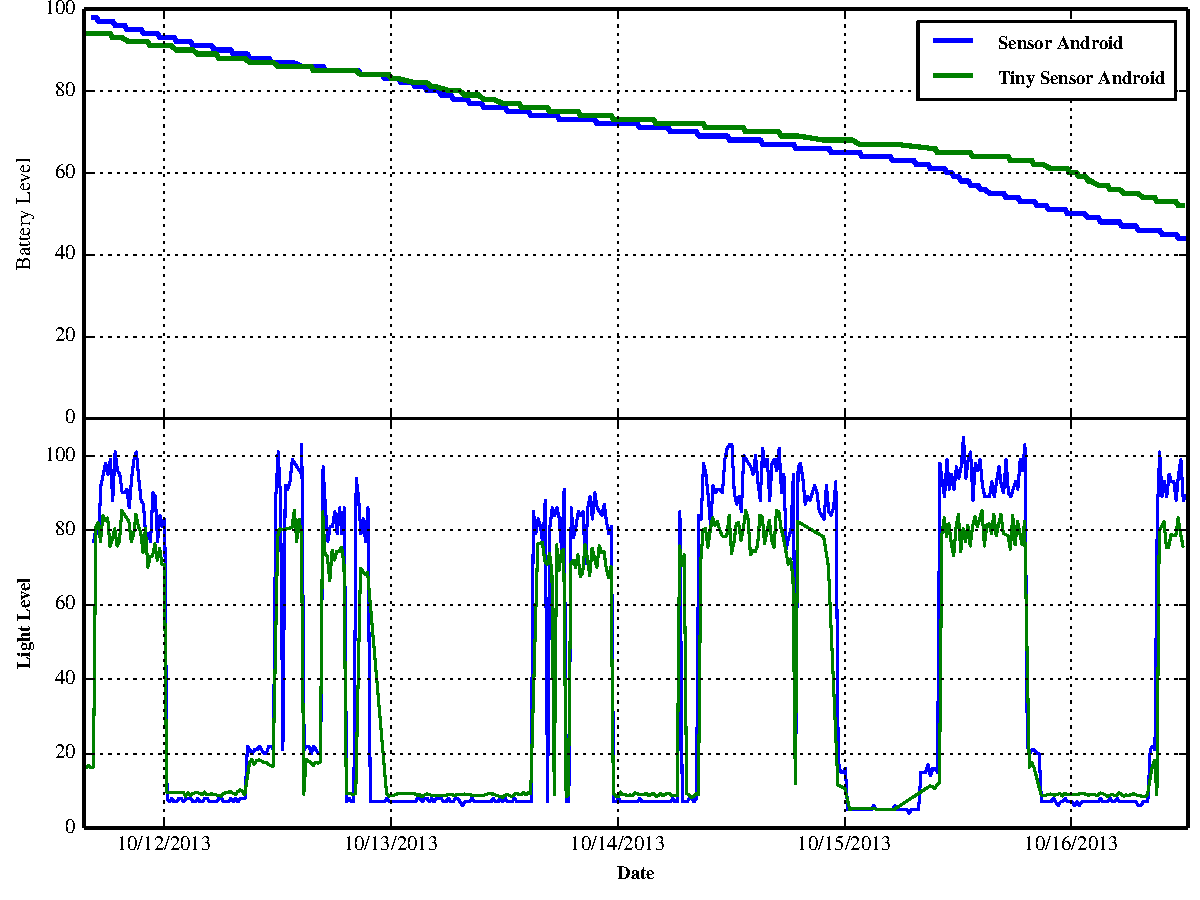
\includegraphics[width=\columnwidth]{./figures/comparison.pdf}

\vspace*{-0.1in}

\caption{\small Lifetime results for two light sensing applications.
\textnormal{Both approaches could achieve an 8--9 day lifetime.}}

\vspace*{-0.1in}

\label{fig-comparison}
\end{figure}

Broadly speaking the teams explored two different options with important
implications for reuse: starting with a stock AOSP platform build and the
familiar Android API, or using a super-minimal Tiny Android build that
discards most of the platform components. We refer to the first approach as
``Sensor Android'' and the second as ``Tiny Sensor Android''. From a
programming perspective, we were hopeful that we could preserve the familiar
Android environment that many programmers today are learning. But from an
energy management perspective, we were worried that the platform contained
features designed around short lifetimes that would prove unhelpful.

Overall we were pleased to discover that both approaches were able to achieve
8--9 days of lifetime on a full battery, as shown in
Figure~\ref{fig-comparison}, despite each approach suffering from a
significant limitation affecting its performance. We believe that this
lifetime may allow perpetual operation with commercially-available solar
panels and are planning to test this assumption as future work. We describe
both approaches and our findings in more detail below.

\subsection{Tiny Sensor Android}
\label{subsec-tiny}

Tiny Android is a development option enabling a stripped-down build intended
for testing new devices, and was not suitable for our application without
modifications. Wifi drivers along with \texttt{dhcpcd} and
\texttt{wpa-supplicant} had to be added to the build process. The only
dependency introduced was \texttt{openssl}. The total package count was
increased by 6, from 11 to 17. The implementation is primarily in C,
consisting of 1500~lines-of-code (LOC). With the smartphone configured with a
static IP address, during each loop iteration an alarm is set to wake up for
the next sample. Then, the light sensor is enabled and a sample is obtained
from the sensor as well as the battery. The Wifi interface is then enabled
for a short period to send the message and disabled immediately after. The
kernel is then asked to suspend the device until it is woken up by the alarm.
Measurements showed that each iteration kept the device awake for
approximately one second.

Figure~\ref{fig-traces} shows current output for one sense-and-send cycle of
our sensing application on Tiny Sensor Android. While the sensing and
transmission complete quickly, allowing the phone to rapidly return to idle,
there was an extra 8~mA of current during the idle state which we have yet to
explain. This experience demonstrates the difficulty of working with a
stripped-down Tiny Android build, which does not fully enter sleep mode
despite receiving commands identical to those provided by the full AOSP
platform.

\begin{figure}[t]
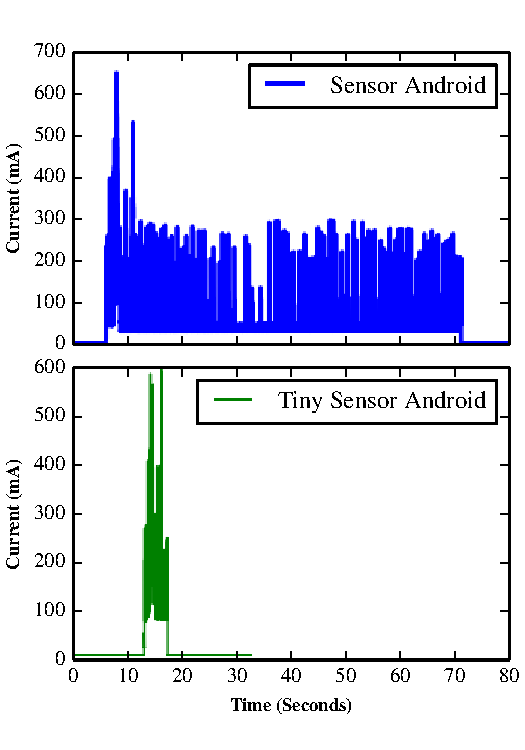
\includegraphics[width=\columnwidth]{./figures/traces.pdf}

\caption{\small Current draw for a single sense-and-send cycle.
\textnormal{Flaws in both approaches are visible. Tiny Sensor Android sleeps
at a high 8~mA, whereas Sensor Android does not return to sleep for almost
one minute.}}

\label{fig-traces}
\end{figure}


\subsection{Sensor Android}
\label{subsec-full}

The image for the Sensor Android build was built from the latest available
AOSP code from the JRO03R branch. No changes were made to the platform as we
wanted to measure stock performance. However, we manually disabled all the
default apps---Browser, Calendar, Email---through the settings to eliminate
any background services the might spawn. (An Android platform designed around
programming sensors would not include these applications in the first place.)
The sensing application was written in 291 LOC using the standard Android
API's for accessing sensors and using the network. Before the start of the
experiment, we assigned a static IP to the Wifi interface and the phone was
put into airplane mode to disable the cellular radio interface. The sensing
application controlled the enabling and disabling of the Wifi radio interface
for each sensing period.

Figure~\ref{fig-traces} shows the current output for one sense-and-send cycle
of our sensing application on Sensor Android. While it completes the
sense-and-send operation as quickly as Tiny Sensor Android and sleeps in the
lowest-power state, there is a 60~s delay before the phone reaches the idle
state. On further investigation, we found that the
\textit{ConnectivityService} in the Android framework was keeping the phone
awake to allow other radio interfaces to connect to a network after one of
the interfaces is disconnected. For our sensing application this is not
required and the platform code can be easily modified to disable this
behavior.

\begin{comment}

% 18 Oct 2013 : GWA : Removed to create space.

\subsection{Expected Lifetime}

Smartphones come with high capacity batteries to power the various components
of the smartphone and enable it to be used for a reasonable amount of time by
the user before it is recharged. Given the fact that we are not using most of
the power hungry components like the Display, GPS, etc. in our sensing
application, we expect to see a long lifetime for our application on a fully
charged battery. Based on the power measurements conducted for each of the
three phases of the application \textit{Idle}, \textit{Sense} and
\textit{Transmit} we model the expected lifetime achievable for a sensing
application in Equation ~\ref{label_exptime}
\begin{equation}\label{label_exptime} E(T)_{hrs} = \frac{C_{Batt}}{I_{idle} +
s*I_{sense}} \end{equation} where:

{\small
\begin{itemize}[label=]
    \item $E(T)_{hrs}$: Expected time in hours.
    \item $C_{Batt}$: Capacity of the battery in mAH.
    \item $I_{idle}$: Idle current draw in mA.
    \item $I_{sense}$: Sensing and transmit current draw in mA.
    \item $s$: hourly sensing rate.
\end{itemize}
}

The average current draw values measured in our experiments were
$I_{idle}=1.56mA$, $I_{sense}=84.06$\footnote{The value excludes the current
draw in the observed long tail.} over a period of 5.3 seconds. With a 1500mAH
battery and a sensing rate of every 15 minutes, the expected lifetime for our
sensing application would be 426.13 Hours. This translates to approximately
18 days of application lifetime. Considering the non linear discharge rate of
the battery as seen in Figure~\ref{fig-comparison}, the expected life would
be less than the calculated value.


\end{comment}

\subsection{Discussion}

Overall we found our results encouraging, particularly the fact that an
unmodified stock Android platform could equal the performance of the
stripped-down Tiny Android build. We believe that this indicates that the
Java programming framework used by Android is efficient enough to use to
program discarded devices, even ones with energy constraints. In addition,
our estimates indicate that fixing the long-tail problem on the Sensor
Android approach will double its lifetime, from 8 days to almost 18.

Inspired by our results we are beginning the process of designing a dedicated
Android build for sensor programming and discarded device reuse. Because many
of these use cases consist primarily of a single application controlling the
entire device, we can disable all extra included applications, as well as
reduce resource limitations such as memory limits. Ideally we would like to
remove all unnecessary platform components as well by examining the
applications usage of the Android API, but our attempts to do this manually
demonstrated that dependencies exist which must be carefully identified.
